\section*{Zadanie 29.}
\begin{task}
Fala płaska biegnąca w kierunku \textsl{Ox} i spolaryzowana liniowo tak, że pole elektryczne jest równoległe do
osi \textsl{Oy} i ma amplitudę 1V/m, pada prostopadle na płytę idealnie przewodzącą, umieszczoną w 
płaszczyźnie x=0. Zapisać rzeczywistą postać wyrażeń na pole \textsl{E} i \textsl{H} dla fali padającej,
odbitej i przechodzącej. Obliczyć gęstość powierzchniową prądu płynącego po płycie. Narysować obwiednie dla
pola \textsl{E} i \textsl{H}. Wyjaśnić, co zmieni się, gdy płyta będzie miala przewodność właściwą $\sigma$
dużą, ale ograniczoną. Narysować obwiednie pól \textsl{E} i \textsl{H} w płycie dla dwóch różnych wartości 
$\sigma_{1}$ oraz $\sigma_{2}=2\sigma_{1}$.\\ \\
\end{task}

\begin{solution}
Postać rzeczywista \textsl{E} i \textsl{H}:
\begin{itemize}
\item $\vec{E^{+}_{1}}=\vec{i_{y}}E_{0}cos(wt-\beta x)$\\
       $\vec{E^{-}_{1}}=-\vec{i_{y}}E_{0}cos(wt+\beta x)$\\
       $\vec{E_{2}}=0$
\item $\vec{H^{+}_{1}}=\vec{i_{z}}H_{0}cos(wt-\beta x)$\\
       $\vec{H^{-}_{1}}=\vec{i_{z}}H_{0}cos(wt+\beta x)$\\
       $\vec{H_{2}}=0$\\ \\
\end{itemize}

Obwiednia pól dla idealnego przewodnika:\\
\begin{center}
$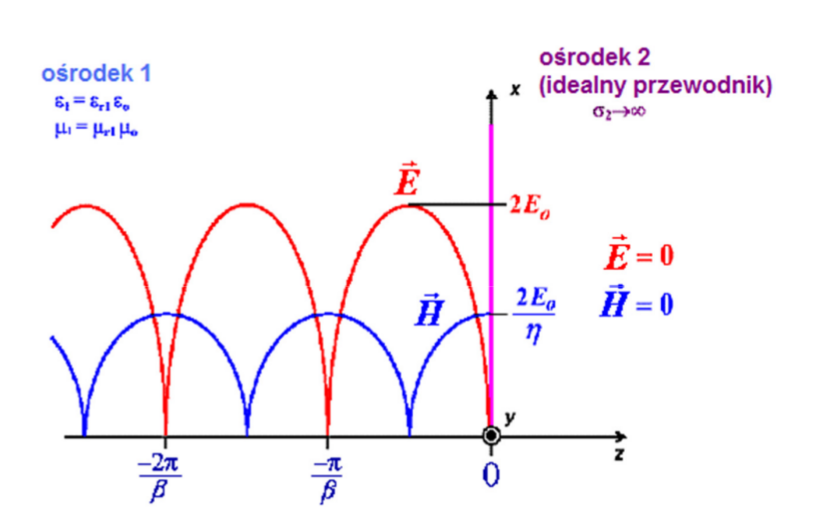
\includegraphics[scale=0.7]{29_1}$\\
\end{center}

Obliczamy gęstość prądu:
$$\vec{n}\times(\vec{H_{2}} - \vec{H_{1}})=\vec{J}$$
$$\vec{H_{2}} = 0$$
$$H_{0} = J$$
Dla wartości $\sigma_{1}$ odwiednia pól \textsl{E} i \textsl{H} maleje wolniej niż dla wartości
$\sigma_{2}=2\sigma_{1}$.\\
Rozkład amplitud dla przykładowej wartości $\sigma$:
\begin{center}
$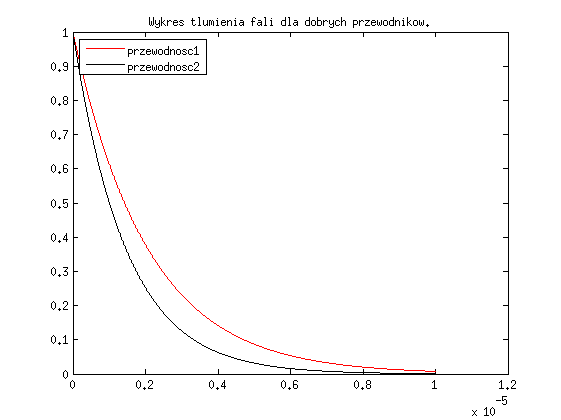
\includegraphics[scale=0.9]{29_2}$\\
\end{center}

\end{solution}
